
%(BEGIN_QUESTION)
% Copyright 2008, Tony R. Kuphaldt, released under the Creative Commons Attribution License (v 1.0)
% This means you may do almost anything with this work of mine, so long as you give me proper credit

A potable (drinking) water storage tank requires a high-level alarm to warn operations personnel of impending overflow conditions.  A high-level switch is on order, but until this switch arrives for installation, you are asked to devise a very simple yet effective high-level indicator device that will function in the interim.

Explain how you would build such a device.  Bonus points for devising a method that uses very simple parts (easily found in a maintenance shop).

\underbar{file i03592}
%(END_QUESTION)





%(BEGIN_ANSWER)

Since the process liquid is potable water, it is mildly conductive to electricity.  Virtually any high-level alarm circuit built around one or two electrodes located at the high-water level will suffice.  Here is a sample idea:

$$\includegraphics[width=15.5cm]{i03592x01.eps}$$

%(END_ANSWER)





%(BEGIN_NOTES)

%INDEX% Measurement, level: practical challenge question

%(END_NOTES)


